\documentclass[12pt,a4paper]{scrartcl}
\usepackage[utf8]{inputenc}
\usepackage{mathtools}
\usepackage[english,russian]{babel}
\usepackage{indentfirst}
\usepackage{misccorr}
\usepackage{amsmath}
\usepackage{mathptmx}
\usepackage{physics}

\usepackage{graphicx}

\usepackage[rightcaption]{sidecap}
\usepackage{wrapfig}

\documentclass[11pt]{article}

    \usepackage[breakable]{tcolorbox}
    \usepackage{parskip} % Stop auto-indenting (to mimic markdown behaviour)
    
    \usepackage{iftex}
    \ifPDFTeX
    	\usepackage[T1]{fontenc}
    	\usepackage{mathpazo}
    \else
    	\usepackage{fontspec}
    \fi

    % Basic figure setup, for now with no caption control since it's done
    % automatically by Pandoc (which extracts ![](path) syntax from Markdown).
    \usepackage{graphicx}
    % Maintain compatibility with old templates. Remove in nbconvert 6.0
    \let\Oldincludegraphics\includegraphics
    % Ensure that by default, figures have no caption (until we provide a
    % proper Figure object with a Caption API and a way to capture that
    % in the conversion process - todo).
    \usepackage{caption}
    \DeclareCaptionFormat{nocaption}{}
    \captionsetup{format=nocaption,aboveskip=0pt,belowskip=0pt}

    \usepackage[Export]{adjustbox} % Used to constrain images to a maximum size
    \adjustboxset{max size={0.9\linewidth}{0.9\paperheight}}
    \usepackage{float}
    \floatplacement{figure}{H} % forces figures to be placed at the correct location
    \usepackage{xcolor} % Allow colors to be defined
    \usepackage{enumerate} % Needed for markdown enumerations to work
    \usepackage{geometry} % Used to adjust the document margins
    \usepackage{amsmath} % Equations
    \usepackage{amssymb} % Equations
    \usepackage{textcomp} % defines textquotesingle
    % Hack from http://tex.stackexchange.com/a/47451/13684:
    \AtBeginDocument{%
        \def\PYZsq{\textquotesingle}% Upright quotes in Pygmentized code
    }
    \usepackage{upquote} % Upright quotes for verbatim code
    \usepackage{eurosym} % defines \euro
    \usepackage[mathletters]{ucs} % Extended unicode (utf-8) support
    \usepackage{fancyvrb} % verbatim replacement that allows latex
    \usepackage{grffile} % extends the file name processing of package graphics 
                         % to support a larger range
    \makeatletter % fix for grffile with XeLaTeX
    \def\Gread@@xetex#1{%
      \IfFileExists{"\Gin@base".bb}%
      {\Gread@eps{\Gin@base.bb}}%
      {\Gread@@xetex@aux#1}%
    }
    \makeatother

    % The hyperref package gives us a pdf with properly built
    % internal navigation ('pdf bookmarks' for the table of contents,
    % internal cross-reference links, web links for URLs, etc.)
    \usepackage{hyperref}
    % The default LaTeX title has an obnoxious amount of whitespace. By default,
    % titling removes some of it. It also provides customization options.
    \usepackage{titling}
    \usepackage{longtable} % longtable support required by pandoc >1.10
    \usepackage{booktabs}  % table support for pandoc > 1.12.2
    \usepackage[inline]{enumitem} % IRkernel/repr support (it uses the enumerate* environment)
    \usepackage[normalem]{ulem} % ulem is needed to support strikethroughs (\sout)
                                % normalem makes italics be italics, not underlines
    \usepackage{mathrsfs}
    

    
    % Colors for the hyperref package
    \definecolor{urlcolor}{rgb}{0,.145,.698}
    \definecolor{linkcolor}{rgb}{.71,0.21,0.01}
    \definecolor{citecolor}{rgb}{.12,.54,.11}

    % ANSI colors
    \definecolor{ansi-black}{HTML}{3E424D}
    \definecolor{ansi-black-intense}{HTML}{282C36}
    \definecolor{ansi-red}{HTML}{E75C58}
    \definecolor{ansi-red-intense}{HTML}{B22B31}
    \definecolor{ansi-green}{HTML}{00A250}
    \definecolor{ansi-green-intense}{HTML}{007427}
    \definecolor{ansi-yellow}{HTML}{DDB62B}
    \definecolor{ansi-yellow-intense}{HTML}{B27D12}
    \definecolor{ansi-blue}{HTML}{208FFB}
    \definecolor{ansi-blue-intense}{HTML}{0065CA}
    \definecolor{ansi-magenta}{HTML}{D160C4}
    \definecolor{ansi-magenta-intense}{HTML}{A03196}
    \definecolor{ansi-cyan}{HTML}{60C6C8}
    \definecolor{ansi-cyan-intense}{HTML}{258F8F}
    \definecolor{ansi-white}{HTML}{C5C1B4}
    \definecolor{ansi-white-intense}{HTML}{A1A6B2}
    \definecolor{ansi-default-inverse-fg}{HTML}{FFFFFF}
    \definecolor{ansi-default-inverse-bg}{HTML}{000000}

    % commands and environments needed by pandoc snippets
    % extracted from the output of `pandoc -s`
    \providecommand{\tightlist}{%
      \setlength{\itemsep}{0pt}\setlength{\parskip}{0pt}}
    \DefineVerbatimEnvironment{Highlighting}{Verbatim}{commandchars=\\\{\}}
    % Add ',fontsize=\small' for more characters per line
    \newenvironment{Shaded}{}{}
    \newcommand{\KeywordTok}[1]{\textcolor[rgb]{0.00,0.44,0.13}{\textbf{{#1}}}}
    \newcommand{\DataTypeTok}[1]{\textcolor[rgb]{0.56,0.13,0.00}{{#1}}}
    \newcommand{\DecValTok}[1]{\textcolor[rgb]{0.25,0.63,0.44}{{#1}}}
    \newcommand{\BaseNTok}[1]{\textcolor[rgb]{0.25,0.63,0.44}{{#1}}}
    \newcommand{\FloatTok}[1]{\textcolor[rgb]{0.25,0.63,0.44}{{#1}}}
    \newcommand{\CharTok}[1]{\textcolor[rgb]{0.25,0.44,0.63}{{#1}}}
    \newcommand{\StringTok}[1]{\textcolor[rgb]{0.25,0.44,0.63}{{#1}}}
    \newcommand{\CommentTok}[1]{\textcolor[rgb]{0.38,0.63,0.69}{\textit{{#1}}}}
    \newcommand{\OtherTok}[1]{\textcolor[rgb]{0.00,0.44,0.13}{{#1}}}
    \newcommand{\AlertTok}[1]{\textcolor[rgb]{1.00,0.00,0.00}{\textbf{{#1}}}}
    \newcommand{\FunctionTok}[1]{\textcolor[rgb]{0.02,0.16,0.49}{{#1}}}
    \newcommand{\RegionMarkerTok}[1]{{#1}}
    \newcommand{\ErrorTok}[1]{\textcolor[rgb]{1.00,0.00,0.00}{\textbf{{#1}}}}
    \newcommand{\NormalTok}[1]{{#1}}
    
    % Additional commands for more recent versions of Pandoc
    \newcommand{\ConstantTok}[1]{\textcolor[rgb]{0.53,0.00,0.00}{{#1}}}
    \newcommand{\SpecialCharTok}[1]{\textcolor[rgb]{0.25,0.44,0.63}{{#1}}}
    \newcommand{\VerbatimStringTok}[1]{\textcolor[rgb]{0.25,0.44,0.63}{{#1}}}
    \newcommand{\SpecialStringTok}[1]{\textcolor[rgb]{0.73,0.40,0.53}{{#1}}}
    \newcommand{\ImportTok}[1]{{#1}}
    \newcommand{\DocumentationTok}[1]{\textcolor[rgb]{0.73,0.13,0.13}{\textit{{#1}}}}
    \newcommand{\AnnotationTok}[1]{\textcolor[rgb]{0.38,0.63,0.69}{\textbf{\textit{{#1}}}}}
    \newcommand{\CommentVarTok}[1]{\textcolor[rgb]{0.38,0.63,0.69}{\textbf{\textit{{#1}}}}}
    \newcommand{\VariableTok}[1]{\textcolor[rgb]{0.10,0.09,0.49}{{#1}}}
    \newcommand{\ControlFlowTok}[1]{\textcolor[rgb]{0.00,0.44,0.13}{\textbf{{#1}}}}
    \newcommand{\OperatorTok}[1]{\textcolor[rgb]{0.40,0.40,0.40}{{#1}}}
    \newcommand{\BuiltInTok}[1]{{#1}}
    \newcommand{\ExtensionTok}[1]{{#1}}
    \newcommand{\PreprocessorTok}[1]{\textcolor[rgb]{0.74,0.48,0.00}{{#1}}}
    \newcommand{\AttributeTok}[1]{\textcolor[rgb]{0.49,0.56,0.16}{{#1}}}
    \newcommand{\InformationTok}[1]{\textcolor[rgb]{0.38,0.63,0.69}{\textbf{\textit{{#1}}}}}
    \newcommand{\WarningTok}[1]{\textcolor[rgb]{0.38,0.63,0.69}{\textbf{\textit{{#1}}}}}
    
    
    % Define a nice break command that doesn't care if a line doesn't already
    % exist.
    \def\br{\hspace*{\fill} \\* }
    % Math Jax compatibility definitions
    \def\gt{>}
    \def\lt{<}
    \let\Oldtex\TeX
    \let\Oldlatex\LaTeX
    \renewcommand{\TeX}{\textrm{\Oldtex}}
    \renewcommand{\LaTeX}{\textrm{\Oldlatex}}
    % Document parameters
    % Document title
    \title{fin (1)}
    
    
    
    
    
% Pygments definitions
\makeatletter
\def\PY@reset{\let\PY@it=\relax \let\PY@bf=\relax%
    \let\PY@ul=\relax \let\PY@tc=\relax%
    \let\PY@bc=\relax \let\PY@ff=\relax}
\def\PY@tok#1{\csname PY@tok@#1\endcsname}
\def\PY@toks#1+{\ifx\relax#1\empty\else%
    \PY@tok{#1}\expandafter\PY@toks\fi}
\def\PY@do#1{\PY@bc{\PY@tc{\PY@ul{%
    \PY@it{\PY@bf{\PY@ff{#1}}}}}}}
\def\PY#1#2{\PY@reset\PY@toks#1+\relax+\PY@do{#2}}

\expandafter\def\csname PY@tok@w\endcsname{\def\PY@tc##1{\textcolor[rgb]{0.73,0.73,0.73}{##1}}}
\expandafter\def\csname PY@tok@c\endcsname{\let\PY@it=\textit\def\PY@tc##1{\textcolor[rgb]{0.25,0.50,0.50}{##1}}}
\expandafter\def\csname PY@tok@cp\endcsname{\def\PY@tc##1{\textcolor[rgb]{0.74,0.48,0.00}{##1}}}
\expandafter\def\csname PY@tok@k\endcsname{\let\PY@bf=\textbf\def\PY@tc##1{\textcolor[rgb]{0.00,0.50,0.00}{##1}}}
\expandafter\def\csname PY@tok@kp\endcsname{\def\PY@tc##1{\textcolor[rgb]{0.00,0.50,0.00}{##1}}}
\expandafter\def\csname PY@tok@kt\endcsname{\def\PY@tc##1{\textcolor[rgb]{0.69,0.00,0.25}{##1}}}
\expandafter\def\csname PY@tok@o\endcsname{\def\PY@tc##1{\textcolor[rgb]{0.40,0.40,0.40}{##1}}}
\expandafter\def\csname PY@tok@ow\endcsname{\let\PY@bf=\textbf\def\PY@tc##1{\textcolor[rgb]{0.67,0.13,1.00}{##1}}}
\expandafter\def\csname PY@tok@nb\endcsname{\def\PY@tc##1{\textcolor[rgb]{0.00,0.50,0.00}{##1}}}
\expandafter\def\csname PY@tok@nf\endcsname{\def\PY@tc##1{\textcolor[rgb]{0.00,0.00,1.00}{##1}}}
\expandafter\def\csname PY@tok@nc\endcsname{\let\PY@bf=\textbf\def\PY@tc##1{\textcolor[rgb]{0.00,0.00,1.00}{##1}}}
\expandafter\def\csname PY@tok@nn\endcsname{\let\PY@bf=\textbf\def\PY@tc##1{\textcolor[rgb]{0.00,0.00,1.00}{##1}}}
\expandafter\def\csname PY@tok@ne\endcsname{\let\PY@bf=\textbf\def\PY@tc##1{\textcolor[rgb]{0.82,0.25,0.23}{##1}}}
\expandafter\def\csname PY@tok@nv\endcsname{\def\PY@tc##1{\textcolor[rgb]{0.10,0.09,0.49}{##1}}}
\expandafter\def\csname PY@tok@no\endcsname{\def\PY@tc##1{\textcolor[rgb]{0.53,0.00,0.00}{##1}}}
\expandafter\def\csname PY@tok@nl\endcsname{\def\PY@tc##1{\textcolor[rgb]{0.63,0.63,0.00}{##1}}}
\expandafter\def\csname PY@tok@ni\endcsname{\let\PY@bf=\textbf\def\PY@tc##1{\textcolor[rgb]{0.60,0.60,0.60}{##1}}}
\expandafter\def\csname PY@tok@na\endcsname{\def\PY@tc##1{\textcolor[rgb]{0.49,0.56,0.16}{##1}}}
\expandafter\def\csname PY@tok@nt\endcsname{\let\PY@bf=\textbf\def\PY@tc##1{\textcolor[rgb]{0.00,0.50,0.00}{##1}}}
\expandafter\def\csname PY@tok@nd\endcsname{\def\PY@tc##1{\textcolor[rgb]{0.67,0.13,1.00}{##1}}}
\expandafter\def\csname PY@tok@s\endcsname{\def\PY@tc##1{\textcolor[rgb]{0.73,0.13,0.13}{##1}}}
\expandafter\def\csname PY@tok@sd\endcsname{\let\PY@it=\textit\def\PY@tc##1{\textcolor[rgb]{0.73,0.13,0.13}{##1}}}
\expandafter\def\csname PY@tok@si\endcsname{\let\PY@bf=\textbf\def\PY@tc##1{\textcolor[rgb]{0.73,0.40,0.53}{##1}}}
\expandafter\def\csname PY@tok@se\endcsname{\let\PY@bf=\textbf\def\PY@tc##1{\textcolor[rgb]{0.73,0.40,0.13}{##1}}}
\expandafter\def\csname PY@tok@sr\endcsname{\def\PY@tc##1{\textcolor[rgb]{0.73,0.40,0.53}{##1}}}
\expandafter\def\csname PY@tok@ss\endcsname{\def\PY@tc##1{\textcolor[rgb]{0.10,0.09,0.49}{##1}}}
\expandafter\def\csname PY@tok@sx\endcsname{\def\PY@tc##1{\textcolor[rgb]{0.00,0.50,0.00}{##1}}}
\expandafter\def\csname PY@tok@m\endcsname{\def\PY@tc##1{\textcolor[rgb]{0.40,0.40,0.40}{##1}}}
\expandafter\def\csname PY@tok@gh\endcsname{\let\PY@bf=\textbf\def\PY@tc##1{\textcolor[rgb]{0.00,0.00,0.50}{##1}}}
\expandafter\def\csname PY@tok@gu\endcsname{\let\PY@bf=\textbf\def\PY@tc##1{\textcolor[rgb]{0.50,0.00,0.50}{##1}}}
\expandafter\def\csname PY@tok@gd\endcsname{\def\PY@tc##1{\textcolor[rgb]{0.63,0.00,0.00}{##1}}}
\expandafter\def\csname PY@tok@gi\endcsname{\def\PY@tc##1{\textcolor[rgb]{0.00,0.63,0.00}{##1}}}
\expandafter\def\csname PY@tok@gr\endcsname{\def\PY@tc##1{\textcolor[rgb]{1.00,0.00,0.00}{##1}}}
\expandafter\def\csname PY@tok@ge\endcsname{\let\PY@it=\textit}
\expandafter\def\csname PY@tok@gs\endcsname{\let\PY@bf=\textbf}
\expandafter\def\csname PY@tok@gp\endcsname{\let\PY@bf=\textbf\def\PY@tc##1{\textcolor[rgb]{0.00,0.00,0.50}{##1}}}
\expandafter\def\csname PY@tok@go\endcsname{\def\PY@tc##1{\textcolor[rgb]{0.53,0.53,0.53}{##1}}}
\expandafter\def\csname PY@tok@gt\endcsname{\def\PY@tc##1{\textcolor[rgb]{0.00,0.27,0.87}{##1}}}
\expandafter\def\csname PY@tok@err\endcsname{\def\PY@bc##1{\setlength{\fboxsep}{0pt}\fcolorbox[rgb]{1.00,0.00,0.00}{1,1,1}{\strut ##1}}}
\expandafter\def\csname PY@tok@kc\endcsname{\let\PY@bf=\textbf\def\PY@tc##1{\textcolor[rgb]{0.00,0.50,0.00}{##1}}}
\expandafter\def\csname PY@tok@kd\endcsname{\let\PY@bf=\textbf\def\PY@tc##1{\textcolor[rgb]{0.00,0.50,0.00}{##1}}}
\expandafter\def\csname PY@tok@kn\endcsname{\let\PY@bf=\textbf\def\PY@tc##1{\textcolor[rgb]{0.00,0.50,0.00}{##1}}}
\expandafter\def\csname PY@tok@kr\endcsname{\let\PY@bf=\textbf\def\PY@tc##1{\textcolor[rgb]{0.00,0.50,0.00}{##1}}}
\expandafter\def\csname PY@tok@bp\endcsname{\def\PY@tc##1{\textcolor[rgb]{0.00,0.50,0.00}{##1}}}
\expandafter\def\csname PY@tok@fm\endcsname{\def\PY@tc##1{\textcolor[rgb]{0.00,0.00,1.00}{##1}}}
\expandafter\def\csname PY@tok@vc\endcsname{\def\PY@tc##1{\textcolor[rgb]{0.10,0.09,0.49}{##1}}}
\expandafter\def\csname PY@tok@vg\endcsname{\def\PY@tc##1{\textcolor[rgb]{0.10,0.09,0.49}{##1}}}
\expandafter\def\csname PY@tok@vi\endcsname{\def\PY@tc##1{\textcolor[rgb]{0.10,0.09,0.49}{##1}}}
\expandafter\def\csname PY@tok@vm\endcsname{\def\PY@tc##1{\textcolor[rgb]{0.10,0.09,0.49}{##1}}}
\expandafter\def\csname PY@tok@sa\endcsname{\def\PY@tc##1{\textcolor[rgb]{0.73,0.13,0.13}{##1}}}
\expandafter\def\csname PY@tok@sb\endcsname{\def\PY@tc##1{\textcolor[rgb]{0.73,0.13,0.13}{##1}}}
\expandafter\def\csname PY@tok@sc\endcsname{\def\PY@tc##1{\textcolor[rgb]{0.73,0.13,0.13}{##1}}}
\expandafter\def\csname PY@tok@dl\endcsname{\def\PY@tc##1{\textcolor[rgb]{0.73,0.13,0.13}{##1}}}
\expandafter\def\csname PY@tok@s2\endcsname{\def\PY@tc##1{\textcolor[rgb]{0.73,0.13,0.13}{##1}}}
\expandafter\def\csname PY@tok@sh\endcsname{\def\PY@tc##1{\textcolor[rgb]{0.73,0.13,0.13}{##1}}}
\expandafter\def\csname PY@tok@s1\endcsname{\def\PY@tc##1{\textcolor[rgb]{0.73,0.13,0.13}{##1}}}
\expandafter\def\csname PY@tok@mb\endcsname{\def\PY@tc##1{\textcolor[rgb]{0.40,0.40,0.40}{##1}}}
\expandafter\def\csname PY@tok@mf\endcsname{\def\PY@tc##1{\textcolor[rgb]{0.40,0.40,0.40}{##1}}}
\expandafter\def\csname PY@tok@mh\endcsname{\def\PY@tc##1{\textcolor[rgb]{0.40,0.40,0.40}{##1}}}
\expandafter\def\csname PY@tok@mi\endcsname{\def\PY@tc##1{\textcolor[rgb]{0.40,0.40,0.40}{##1}}}
\expandafter\def\csname PY@tok@il\endcsname{\def\PY@tc##1{\textcolor[rgb]{0.40,0.40,0.40}{##1}}}
\expandafter\def\csname PY@tok@mo\endcsname{\def\PY@tc##1{\textcolor[rgb]{0.40,0.40,0.40}{##1}}}
\expandafter\def\csname PY@tok@ch\endcsname{\let\PY@it=\textit\def\PY@tc##1{\textcolor[rgb]{0.25,0.50,0.50}{##1}}}
\expandafter\def\csname PY@tok@cm\endcsname{\let\PY@it=\textit\def\PY@tc##1{\textcolor[rgb]{0.25,0.50,0.50}{##1}}}
\expandafter\def\csname PY@tok@cpf\endcsname{\let\PY@it=\textit\def\PY@tc##1{\textcolor[rgb]{0.25,0.50,0.50}{##1}}}
\expandafter\def\csname PY@tok@c1\endcsname{\let\PY@it=\textit\def\PY@tc##1{\textcolor[rgb]{0.25,0.50,0.50}{##1}}}
\expandafter\def\csname PY@tok@cs\endcsname{\let\PY@it=\textit\def\PY@tc##1{\textcolor[rgb]{0.25,0.50,0.50}{##1}}}

\def\PYZbs{\char`\\}
\def\PYZus{\char`\_}
\def\PYZob{\char`\{}
\def\PYZcb{\char`\}}
\def\PYZca{\char`\^}
\def\PYZam{\char`\&}
\def\PYZlt{\char`\<}
\def\PYZgt{\char`\>}
\def\PYZsh{\char`\#}
\def\PYZpc{\char`\%}
\def\PYZdl{\char`\$}
\def\PYZhy{\char`\-}
\def\PYZsq{\char`\'}
\def\PYZdq{\char`\"}
\def\PYZti{\char`\~}
% for compatibility with earlier versions
\def\PYZat{@}
\def\PYZlb{[}
\def\PYZrb{]}
\makeatother


    % For linebreaks inside Verbatim environment from package fancyvrb. 
    \makeatletter
        \newbox\Wrappedcontinuationbox 
        \newbox\Wrappedvisiblespacebox 
        \newcommand*\Wrappedvisiblespace {\textcolor{red}{\textvisiblespace}} 
        \newcommand*\Wrappedcontinuationsymbol {\textcolor{red}{\llap{\tiny$\m@th\hookrightarrow$}}} 
        \newcommand*\Wrappedcontinuationindent {3ex } 
        \newcommand*\Wrappedafterbreak {\kern\Wrappedcontinuationindent\copy\Wrappedcontinuationbox} 
        % Take advantage of the already applied Pygments mark-up to insert 
        % potential linebreaks for TeX processing. 
        %        {, <, #, %, $, ' and ": go to next line. 
        %        _, }, ^, &, >, - and ~: stay at end of broken line. 
        % Use of \textquotesingle for straight quote. 
        \newcommand*\Wrappedbreaksatspecials {% 
            \def\PYGZus{\discretionary{\char`\_}{\Wrappedafterbreak}{\char`\_}}% 
            \def\PYGZob{\discretionary{}{\Wrappedafterbreak\char`\{}{\char`\{}}% 
            \def\PYGZcb{\discretionary{\char`\}}{\Wrappedafterbreak}{\char`\}}}% 
            \def\PYGZca{\discretionary{\char`\^}{\Wrappedafterbreak}{\char`\^}}% 
            \def\PYGZam{\discretionary{\char`\&}{\Wrappedafterbreak}{\char`\&}}% 
            \def\PYGZlt{\discretionary{}{\Wrappedafterbreak\char`\<}{\char`\<}}% 
            \def\PYGZgt{\discretionary{\char`\>}{\Wrappedafterbreak}{\char`\>}}% 
            \def\PYGZsh{\discretionary{}{\Wrappedafterbreak\char`\#}{\char`\#}}% 
            \def\PYGZpc{\discretionary{}{\Wrappedafterbreak\char`\%}{\char`\%}}% 
            \def\PYGZdl{\discretionary{}{\Wrappedafterbreak\char`\$}{\char`\$}}% 
            \def\PYGZhy{\discretionary{\char`\-}{\Wrappedafterbreak}{\char`\-}}% 
            \def\PYGZsq{\discretionary{}{\Wrappedafterbreak\textquotesingle}{\textquotesingle}}% 
            \def\PYGZdq{\discretionary{}{\Wrappedafterbreak\char`\"}{\char`\"}}% 
            \def\PYGZti{\discretionary{\char`\~}{\Wrappedafterbreak}{\char`\~}}% 
        } 
        % Some characters . , ; ? ! / are not pygmentized. 
        % This macro makes them "active" and they will insert potential linebreaks 
        \newcommand*\Wrappedbreaksatpunct {% 
            \lccode`\~`\.\lowercase{\def~}{\discretionary{\hbox{\char`\.}}{\Wrappedafterbreak}{\hbox{\char`\.}}}% 
            \lccode`\~`\,\lowercase{\def~}{\discretionary{\hbox{\char`\,}}{\Wrappedafterbreak}{\hbox{\char`\,}}}% 
            \lccode`\~`\;\lowercase{\def~}{\discretionary{\hbox{\char`\;}}{\Wrappedafterbreak}{\hbox{\char`\;}}}% 
            \lccode`\~`\:\lowercase{\def~}{\discretionary{\hbox{\char`\:}}{\Wrappedafterbreak}{\hbox{\char`\:}}}% 
            \lccode`\~`\?\lowercase{\def~}{\discretionary{\hbox{\char`\?}}{\Wrappedafterbreak}{\hbox{\char`\?}}}% 
            \lccode`\~`\!\lowercase{\def~}{\discretionary{\hbox{\char`\!}}{\Wrappedafterbreak}{\hbox{\char`\!}}}% 
            \lccode`\~`\/\lowercase{\def~}{\discretionary{\hbox{\char`\/}}{\Wrappedafterbreak}{\hbox{\char`\/}}}% 
            \catcode`\.\active
            \catcode`\,\active 
            \catcode`\;\active
            \catcode`\:\active
            \catcode`\?\active
            \catcode`\!\active
            \catcode`\/\active 
            \lccode`\~`\~ 	
        }
    \makeatother

    \let\OriginalVerbatim=\Verbatim
    \makeatletter
    \renewcommand{\Verbatim}[1][1]{%
        %\parskip\z@skip
        \sbox\Wrappedcontinuationbox {\Wrappedcontinuationsymbol}%
        \sbox\Wrappedvisiblespacebox {\FV@SetupFont\Wrappedvisiblespace}%
        \def\FancyVerbFormatLine ##1{\hsize\linewidth
            \vtop{\raggedright\hyphenpenalty\z@\exhyphenpenalty\z@
                \doublehyphendemerits\z@\finalhyphendemerits\z@
                \strut ##1\strut}%
        }%
        % If the linebreak is at a space, the latter will be displayed as visible
        % space at end of first line, and a continuation symbol starts next line.
        % Stretch/shrink are however usually zero for typewriter font.
        \def\FV@Space {%
            \nobreak\hskip\z@ plus\fontdimen3\font minus\fontdimen4\font
            \discretionary{\copy\Wrappedvisiblespacebox}{\Wrappedafterbreak}
            {\kern\fontdimen2\font}%
        }%
        
        % Allow breaks at special characters using \PYG... macros.
        \Wrappedbreaksatspecials
        % Breaks at punctuation characters . , ; ? ! and / need catcode=\active 	
        \OriginalVerbatim[#1,codes*=\Wrappedbreaksatpunct]%
    }
    \makeatother

    % Exact colors from NB
    \definecolor{incolor}{HTML}{303F9F}
    \definecolor{outcolor}{HTML}{D84315}
    \definecolor{cellborder}{HTML}{CFCFCF}
    \definecolor{cellbackground}{HTML}{F7F7F7}
    
    % prompt
    \makeatletter
    \newcommand{\boxspacing}{\kern\kvtcb@left@rule\kern\kvtcb@boxsep}
    \makeatother
    \newcommand{\prompt}[4]{
        \ttfamily\llap{{\color{#2}[#3]:\hspace{3pt}#4}}\vspace{-\baselineskip}
    }
    

    
    % Prevent overflowing lines due to hard-to-break entities
    \sloppy 
    % Setup hyperref package
    \hypersetup{
      breaklinks=true,  % so long urls are correctly broken across lines
      colorlinks=true,
      urlcolor=urlcolor,
      linkcolor=linkcolor,
      citecolor=citecolor,
      }
    % Slightly bigger margins than the latex defaults
    
    \geometry{verbose,tmargin=1in,bmargin=1in,lmargin=1in,rmargin=1in}
    

\begin{document}

\begin{titlepage}
  \begin{center}
     
    \vspace{0.5cm}
 
    НОВОСИБИРСКИЙ ГОСУДАРСТВЕННЫЙ УНИВЕРСИТЕТ
    \vspace{0.25cm}
     
    Механико-математический факультет
     
    Кафедра: Математика и компьютерные науки
    \vfill
     
     
    Тлепбергенова Дарья Дулатовна
    \vfill
 
    \textsc{Отчет по вычислительному практикуму}\\[5mm]
     
    {\LARGE Решение двумерного эллиптического уравнения \\
      методом конечных разностей.\\
    Вариант 14.\\[2mm]}
  \bigskip
     
    3 курс, группа 16121
    \end{center}
\vfill
 \newlength{\ML}
\settowidth{\ML}{«\underline{\hspace{0.7cm}}» \underline{\hspace{2cm}}}
    \hfill\begin{minipage}{0.4\textwidth}
     Преподаватель:\\
    Махоткин Олег Александрович
    \end{minipage}%
\bigskip

 \vfill
\begin{center}
  Новосибирск, 2018 г.
\end{center}
\end{titlepage}

\newpage

\section{Постановка задачи.}

С помощью 5-точечной схемы свести уравнение задачи Дирихле

\[
    -a{\dfrac{{\partial}^2 u}{\partial x^{2}}}-b{\dfrac{{\partial}^2 u}{\partial y^{2}}}=f(x,y), (x,y)\in D 
\]

\[
    u(x,y)= \varphi(x,y), (x,y)\in \partial D
\]

в области $D$ к решению системы линейных алгебраических уравнений $ Az = F $.
Использовать разностную схему с шагами:

\[
    h_x=h_y=h=\frac{1}{m}
\]

\[
    -a\dfrac{U_{i-1,j}-2U_{i,j}+U_{i+1,j}}{h^2}-b\dfrac{U_{i,j-1}-2U_{i,j}+U_{i,j+1}}{h^2}=f_{i,j}
\]

Для

\[
    a=1; b=1
\]

\[
    f(x,y)=2\pi^2sin(\pi x)sin(\pi x),
\]

\[
     \varphi(x,y)=sin(\pi x)sin(\pi x)
\]

Область $D$ выглядит следующим образом:

\begin{figure}[h]
    \centering
    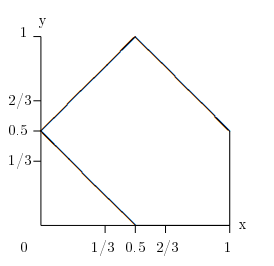
\includegraphics[width=6cm]{img/domain.png}
\end{figure}

\begin{enumerate}
    \item Найти погрешность аппроксимации разностной схемы на решении краевой задачи.
    \item Проверить, что функция $  \varphi(x,y)$ является точным решением краевой задачи.
    \item Для небольшого числа узлов сетки и двух вариантов нумерации внутренних узлов выписать в симметрическом виде матрицы $A$. Убедиться, что они являются симметричными и разреженными.
    \item Записать полученные матрицы в упакованном виде (по строкам).
    \item Найти максимальное и минимальное собственное значения матрицы $A$ для нескольких значений $m$ степенным методом.
    \item Используя собственные значения оператора $(Lv)_i=v_{i-1}-2v_i+v_{i+1},i=1,...,m-1, v_0=v_m=0$, найти собственные значения двумерного разностного оператора рассматриваемой задачи для $D=Q^2=[0,1]^2$. Сравнивать полученное значение $\lambda_{min}(h)$ с $\lambda_{min}$ для дифференциальной задачи. Получить асимптотическое разложение $\lambda_{min}(h)$ по $h$.
    \item Найти решение системы уравнений $Az=F$ методом установления и методом верхней релаксации.
    \item Для нескольких значений числа интервалов $m$ найти относительные погрешности разностного решения $	\Delta=<|U(x,y)-\varphi(x,y)|>/<|\varphi(x,y)|>.$
    
    Здесь $<|g(x,y)|>=\sum_{i,j}[(i,j)=\in D]|g(x_i,y_j)|.$
    \item Вывести на экран разностное решение $U(x,y)$ и погрешность $U(x,y)-\varphi(x,y)$.
    
\end{enumerate}

\section{Исследование данной схемы на точность и устойчивость.}

    \subsection{Погрешность аппроксимации.}
    Оценим погрешность аппроксимации данной задачи, для этого, Приблизим оператор Лапласа разностным оператором:
    \[
        \Lambda u = \Lambda_1 u + \Lambda_2 u = u_{x,x}+u_{y,y}
    \]
    Тогда с помощью разложения в ряд Тейлора получаем:
    \[
        \Lambda_1 u = {\dfrac{{\partial}^2 u}{\partial x^{2}}}+\dfrac{h^2}{12}{\dfrac{{\partial}^4 u}{\partial x^{4}}}+O(h^4)
    \]
    \[
         \Lambda_2 u = {\dfrac{{\partial}^2 u}{\partial y^{2}}}+\dfrac{h^2}{12}{\dfrac{{\partial}^4 u}{\partial y^{4}}}+O(h^4)
    \]
    Тогда
    \[
        \Lambda u - \Delta v = \dfrac{h^2}{12}{\dfrac{{\partial}^4 u}{\partial x^{4}}}+\dfrac{h^2}{12}{\dfrac{{\partial}^4 u}{\partial y^{4}}}+O(h^4)
    \]
    Отсюда следует, что
    \[
        \Lambda u - \Delta v = O(h^2)
    \]
    Таким образом, данный разностный оператор аппроксимирует оператор Лапласа со  вторым порядком аппроксимации на регулярном шаблоне "крест". 
    
\newpage

\section{Описание вычислительного метода. Алгоритм решения программы.}
\begin{itemize}
	\item Изобразим шаблон нашей схемы:
	\begin{figure}[h]
		\centering
		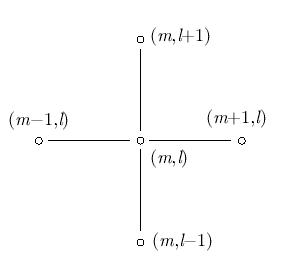
\includegraphics[width=6cm]{img/scheme.jpg}
	\end{figure}
	\item Наложим на нашу область равномерную сетку с шагом $h$     и пронумеруем узлы сетки следующим образом:
	\begin{figure}[h]
		\centering
		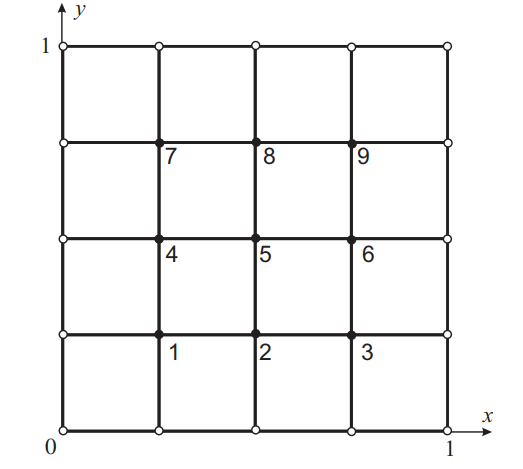
\includegraphics[width=6cm]{img/normal.png}
	\end{figure}
	\item С помощью отдельной функции, отделим точки, принадлежащие границе области D, точки, лежащие строго внутри области D и точки не принадлежащие области.  
	\item Для граничных точек сразу вычисляем значения искомой функции
	\item Для всех внутренних точек выполняем разностную схему и ищем их значения, как решение СЛАУ.На основе этого получаем матрицу.
	\item Записываем эту матрицу в упакованном виде
	\item Ищем у полученной матрицы max и min числа
	\item Решаем матрицу (СЛАУ) с помощью метода верхней релаксации и методом установления
	\item Заносим оставшиеся значения в матрицу решений и выводим полученный график
\end{itemize} 

\section{Код программы}


    \begin{tcolorbox}[breakable, size=fbox, boxrule=1pt, pad at break*=1mm,colback=cellbackground, colframe=cellborder]
\prompt{In}{incolor}{1}{\boxspacing}
\begin{Verbatim}[commandchars=\\\{\}]
\PY{c+c1}{\PYZsh{}\PYZpc{}matplotlib inline}
\PY{o}{\PYZpc{}}\PY{k}{matplotlib} notebook
\end{Verbatim}
\end{tcolorbox}

    \begin{tcolorbox}[breakable, size=fbox, boxrule=1pt, pad at break*=1mm,colback=cellbackground, colframe=cellborder]
\prompt{In}{incolor}{2}{\boxspacing}
\begin{Verbatim}[commandchars=\\\{\}]
\PY{k+kn}{import} \PY{n+nn}{math}
\PY{k+kn}{import} \PY{n+nn}{numpy} \PY{k}{as} \PY{n+nn}{np}
\PY{k+kn}{import} \PY{n+nn}{scipy}\PY{n+nn}{.}\PY{n+nn}{linalg} \PY{k}{as} \PY{n+nn}{sla}
\PY{k+kn}{import} \PY{n+nn}{matplotlib}\PY{n+nn}{.}\PY{n+nn}{pyplot} \PY{k}{as} \PY{n+nn}{plt}
\PY{k+kn}{from} \PY{n+nn}{scipy}\PY{n+nn}{.}\PY{n+nn}{sparse} \PY{k+kn}{import} \PY{n}{csc\PYZus{}matrix}
\PY{k+kn}{from} \PY{n+nn}{scipy}\PY{n+nn}{.}\PY{n+nn}{sparse} \PY{k+kn}{import} \PY{n}{csr\PYZus{}matrix}
\PY{k+kn}{from} \PY{n+nn}{scipy} \PY{k+kn}{import} \PY{n}{sparse}
\PY{k+kn}{import} \PY{n+nn}{scipy}
\PY{k+kn}{import} \PY{n+nn}{scipy}\PY{n+nn}{.}\PY{n+nn}{sparse}\PY{n+nn}{.}\PY{n+nn}{linalg} \PY{k}{as} \PY{n+nn}{linalg}

\PY{k+kn}{from} \PY{n+nn}{mpl\PYZus{}toolkits}\PY{n+nn}{.}\PY{n+nn}{mplot3d} \PY{k+kn}{import} \PY{n}{Axes3D}
\PY{k+kn}{from} \PY{n+nn}{matplotlib} \PY{k+kn}{import} \PY{n}{cm}
\PY{k+kn}{from} \PY{n+nn}{matplotlib}\PY{n+nn}{.}\PY{n+nn}{ticker} \PY{k+kn}{import} \PY{n}{LinearLocator}\PY{p}{,} \PY{n}{FormatStrFormatter}
\end{Verbatim}
\end{tcolorbox}

    \begin{tcolorbox}[breakable, size=fbox, boxrule=1pt, pad at break*=1mm,colback=cellbackground, colframe=cellborder]
\prompt{In}{incolor}{3}{\boxspacing}
\begin{Verbatim}[commandchars=\\\{\}]
\PY{n}{a} \PY{o}{=} \PY{l+m+mi}{1}
\PY{n}{b} \PY{o}{=} \PY{l+m+mi}{1}
\PY{n}{m} \PY{o}{=} \PY{l+m+mi}{4}
\PY{n}{h} \PY{o}{=} \PY{l+m+mi}{1} \PY{o}{/} \PY{n}{m}
\PY{n}{eps} \PY{o}{=} \PY{l+m+mf}{1e\PYZhy{}9}
\PY{n}{number} \PY{o}{=} \PY{n}{np}\PY{o}{.}\PY{n}{zeros}\PY{p}{(}\PY{p}{(}\PY{n}{m} \PY{o}{+} \PY{l+m+mi}{1}\PY{p}{,} \PY{n}{m} \PY{o}{+} \PY{l+m+mi}{1}\PY{p}{)}\PY{p}{,} \PY{n}{dtype} \PY{o}{=} \PY{n+nb}{int}\PY{p}{)}
\end{Verbatim}
\end{tcolorbox}

    \begin{tcolorbox}[breakable, size=fbox, boxrule=1pt, pad at break*=1mm,colback=cellbackground, colframe=cellborder]
\prompt{In}{incolor}{4}{\boxspacing}
\begin{Verbatim}[commandchars=\\\{\}]
\PY{k}{def} \PY{n+nf}{check\PYZus{}in}\PY{p}{(}\PY{n}{x}\PY{p}{,} \PY{n}{y}\PY{p}{)}\PY{p}{:} \PY{c+c1}{\PYZsh{}function of checking }
        \PY{k}{return} \PY{p}{(}\PY{p}{(}\PY{p}{(}\PY{o}{\PYZhy{}}\PY{n}{x} \PY{o}{+} \PY{l+m+mf}{0.5}\PY{p}{)} \PY{o}{\PYZlt{}} \PY{n}{y}\PY{p}{)} \PY{o+ow}{and} \PY{p}{(}\PY{p}{(}\PY{n}{x} \PY{o}{+} \PY{l+m+mf}{0.5}\PY{p}{)} \PY{o}{\PYZgt{}} \PY{n}{y}\PY{p}{)} \PY{o+ow}{and}
                \PY{p}{(}\PY{p}{(}\PY{o}{\PYZhy{}}\PY{n}{x} \PY{o}{+} \PY{l+m+mf}{1.5}\PY{p}{)} \PY{o}{\PYZgt{}} \PY{n}{y}\PY{p}{)} \PY{o+ow}{and} \PY{p}{(}\PY{n}{x} \PY{o}{\PYZlt{}} \PY{l+m+mi}{1}\PY{p}{)} \PY{o+ow}{and} \PY{p}{(}\PY{n}{y} \PY{o}{\PYZgt{}} \PY{l+m+mi}{0}\PY{p}{)}\PY{p}{)}
\end{Verbatim}
\end{tcolorbox}

    \begin{tcolorbox}[breakable, size=fbox, boxrule=1pt, pad at break*=1mm,colback=cellbackground, colframe=cellborder]
\prompt{In}{incolor}{5}{\boxspacing}
\begin{Verbatim}[commandchars=\\\{\}]
\PY{k}{def} \PY{n+nf}{check\PYZus{}border}\PY{p}{(}\PY{n}{x}\PY{p}{,}\PY{n}{y}\PY{p}{)}\PY{p}{:}
    \PY{k}{return} \PY{p}{(}\PY{n}{x} \PY{o}{\PYZgt{}}\PY{o}{=} \PY{l+m+mi}{0}\PY{p}{)} \PY{o+ow}{and} \PY{p}{(}\PY{n}{y} \PY{o}{\PYZgt{}}\PY{o}{=} \PY{l+m+mi}{0}\PY{p}{)} \PY{o+ow}{and} \PY{p}{(}\PY{n}{x} \PY{o}{\PYZlt{}}\PY{o}{=} \PY{l+m+mi}{1}\PY{p}{)} \PY{o+ow}{and} \PY{p}{(}\PY{n}{y} \PY{o}{\PYZlt{}}\PY{o}{=} \PY{l+m+mi}{1}\PY{p}{)} \PY{o+ow}{and} \PY{p}{(}\PY{p}{(}\PY{p}{(}\PY{o}{\PYZhy{}}\PY{n}{x} \PY{o}{+} \PY{l+m+mf}{0.5}\PY{p}{)} \PY{o}{==} \PY{n}{y}\PY{p}{)} \PY{o+ow}{or} \PY{p}{(}\PY{p}{(}\PY{n}{x} \PY{o}{+} \PY{l+m+mf}{0.5}\PY{p}{)} \PY{o}{==} \PY{n}{y}\PY{p}{)} \PY{o+ow}{or} \PY{p}{(}\PY{p}{(}\PY{o}{\PYZhy{}}\PY{n}{x} \PY{o}{+} \PY{l+m+mf}{1.5}\PY{p}{)} \PY{o}{==} \PY{n}{y}\PY{p}{)} \PY{o+ow}{or} \PY{p}{(}\PY{p}{(}\PY{n}{x} \PY{o}{==} \PY{l+m+mi}{1}\PY{p}{)} \PY{o+ow}{and} \PY{p}{(}\PY{n}{y} \PY{o}{\PYZlt{}}\PY{o}{=} \PY{l+m+mf}{0.5}\PY{p}{)}\PY{p}{)} \PY{o+ow}{or} \PY{p}{(}\PY{p}{(}\PY{n}{y} \PY{o}{==} \PY{l+m+mi}{0}\PY{p}{)} \PY{o+ow}{and} \PY{p}{(}\PY{n}{x} \PY{o}{\PYZgt{}}\PY{o}{=} \PY{l+m+mf}{0.5}\PY{p}{)}\PY{p}{)}\PY{p}{)}\PY{p}{;}
\end{Verbatim}
\end{tcolorbox}

    \begin{tcolorbox}[breakable, size=fbox, boxrule=1pt, pad at break*=1mm,colback=cellbackground, colframe=cellborder]
\prompt{In}{incolor}{6}{\boxspacing}
\begin{Verbatim}[commandchars=\\\{\}]
\PY{k}{def} \PY{n+nf}{f}\PY{p}{(}\PY{n}{x}\PY{p}{,} \PY{n}{y}\PY{p}{)}\PY{p}{:}
    \PY{k}{return} \PY{l+m+mf}{2.0} \PY{o}{*} \PY{n}{math}\PY{o}{.}\PY{n}{pi} \PY{o}{*} \PY{n}{math}\PY{o}{.}\PY{n}{pi} \PY{o}{*} \PY{n}{math}\PY{o}{.}\PY{n}{sin}\PY{p}{(}\PY{n}{math}\PY{o}{.}\PY{n}{pi} \PY{o}{*} \PY{n}{x}\PY{p}{)} \PY{o}{*} \PY{n}{math}\PY{o}{.}\PY{n}{sin}\PY{p}{(}\PY{n}{math}\PY{o}{.}\PY{n}{pi} \PY{o}{*} \PY{n}{y}\PY{p}{)}

\PY{k}{def} \PY{n+nf}{phi}\PY{p}{(}\PY{n}{x}\PY{p}{,} \PY{n}{y}\PY{p}{)}\PY{p}{:}
    \PY{k}{return} \PY{n}{math}\PY{o}{.}\PY{n}{sin}\PY{p}{(}\PY{n}{math}\PY{o}{.}\PY{n}{pi} \PY{o}{*} \PY{n}{x}\PY{p}{)} \PY{o}{*} \PY{n}{math}\PY{o}{.}\PY{n}{sin}\PY{p}{(}\PY{n}{math}\PY{o}{.}\PY{n}{pi} \PY{o}{*} \PY{n}{y}\PY{p}{)}
\end{Verbatim}
\end{tcolorbox}

    \begin{tcolorbox}[breakable, size=fbox, boxrule=1pt, pad at break*=1mm,colback=cellbackground, colframe=cellborder]
\prompt{In}{incolor}{7}{\boxspacing}
\begin{Verbatim}[commandchars=\\\{\}]
\PY{n}{cnt} \PY{o}{=} \PY{l+m+mi}{0}
\PY{k}{for} \PY{n}{i} \PY{o+ow}{in} \PY{n+nb}{range}\PY{p}{(}\PY{l+m+mi}{1}\PY{p}{,} \PY{n}{m}\PY{p}{)}\PY{p}{:}
    \PY{k}{for} \PY{n}{j} \PY{o+ow}{in} \PY{n+nb}{range}\PY{p}{(}\PY{l+m+mi}{1}\PY{p}{,} \PY{n}{m}\PY{p}{)}\PY{p}{:}
        \PY{k}{if} \PY{n}{check\PYZus{}in}\PY{p}{(}\PY{n}{i} \PY{o}{/} \PY{n}{m}\PY{p}{,} \PY{n}{j} \PY{o}{/} \PY{n}{m}\PY{p}{)}\PY{p}{:}
            \PY{n}{number}\PY{p}{[}\PY{n}{i}\PY{p}{]}\PY{p}{[}\PY{n}{j}\PY{p}{]} \PY{o}{=} \PY{n}{cnt}
            \PY{n}{cnt} \PY{o}{+}\PY{o}{=} \PY{l+m+mi}{1}
\end{Verbatim}
\end{tcolorbox}

    \begin{tcolorbox}[breakable, size=fbox, boxrule=1pt, pad at break*=1mm,colback=cellbackground, colframe=cellborder]
\prompt{In}{incolor}{8}{\boxspacing}
\begin{Verbatim}[commandchars=\\\{\}]
\PY{n}{x} \PY{o}{=} \PY{n}{np}\PY{o}{.}\PY{n}{zeros}\PY{p}{(}\PY{p}{(}\PY{n}{m} \PY{o}{+} \PY{l+m+mi}{1}\PY{p}{,} \PY{n}{m} \PY{o}{+} \PY{l+m+mi}{1}\PY{p}{)}\PY{p}{)}
\PY{n}{y} \PY{o}{=} \PY{n}{np}\PY{o}{.}\PY{n}{zeros}\PY{p}{(}\PY{p}{(}\PY{n}{m} \PY{o}{+} \PY{l+m+mi}{1}\PY{p}{,} \PY{n}{m} \PY{o}{+} \PY{l+m+mi}{1}\PY{p}{)}\PY{p}{)}
\PY{n}{indicate} \PY{o}{=} \PY{n}{np}\PY{o}{.}\PY{n}{zeros}\PY{p}{(}\PY{p}{(}\PY{n}{m} \PY{o}{+} \PY{l+m+mi}{1}\PY{p}{,}\PY{n}{m} \PY{o}{+} \PY{l+m+mi}{1}\PY{p}{)}\PY{p}{,}\PY{n}{dtype} \PY{o}{=} \PY{n+nb}{int}\PY{p}{)}
\PY{n}{x1} \PY{o}{=} \PY{l+m+mi}{0}
\PY{n}{y1} \PY{o}{=} \PY{l+m+mi}{0}
\PY{n}{k} \PY{o}{=} \PY{l+m+mi}{0}

\PY{k}{for} \PY{n}{i} \PY{o+ow}{in} \PY{n+nb}{range}\PY{p}{(}\PY{l+m+mi}{1}\PY{p}{,} \PY{n}{m} \PY{o}{+} \PY{l+m+mi}{1}\PY{p}{)}\PY{p}{:}
    \PY{k}{for} \PY{n}{j} \PY{o+ow}{in} \PY{n+nb}{range}\PY{p}{(}\PY{l+m+mi}{1}\PY{p}{,} \PY{n}{m} \PY{o}{+} \PY{l+m+mi}{1}\PY{p}{)}\PY{p}{:}
        \PY{n}{x}\PY{p}{[}\PY{n}{i}\PY{p}{]}\PY{p}{[}\PY{n}{j}\PY{p}{]} \PY{o}{=} \PY{n}{i} \PY{o}{/} \PY{n}{m}
        \PY{n}{y}\PY{p}{[}\PY{n}{i}\PY{p}{]}\PY{p}{[}\PY{n}{j}\PY{p}{]} \PY{o}{=} \PY{n}{j} \PY{o}{/} \PY{n}{m}
        
\PY{k}{for} \PY{n}{i} \PY{o+ow}{in} \PY{n+nb}{range}\PY{p}{(}\PY{l+m+mi}{0}\PY{p}{,} \PY{n}{m} \PY{o}{+} \PY{l+m+mi}{1}\PY{p}{)}\PY{p}{:}
    \PY{n}{x1}\PY{o}{=}\PY{l+m+mi}{0}
    \PY{k}{for} \PY{n}{j} \PY{o+ow}{in} \PY{n+nb}{range}\PY{p}{(}\PY{l+m+mi}{0}\PY{p}{,} \PY{n}{m} \PY{o}{+} \PY{l+m+mi}{1}\PY{p}{)}\PY{p}{:}
        \PY{k}{if} \PY{p}{(}\PY{n}{check\PYZus{}in}\PY{p}{(}\PY{n}{x1}\PY{p}{,}\PY{n}{y1}\PY{p}{)}\PY{p}{)}\PY{p}{:}
            \PY{n}{indicate}\PY{p}{[}\PY{n}{i}\PY{p}{]}\PY{p}{[}\PY{n}{j}\PY{p}{]} \PY{o}{=} \PY{n}{k}
            \PY{n}{k}\PY{o}{=}\PY{n}{k}\PY{o}{+}\PY{l+m+mi}{1}
        \PY{k}{else} \PY{p}{:}
            \PY{k}{if} \PY{p}{(}\PY{n}{check\PYZus{}border}\PY{p}{(}\PY{n}{x1}\PY{p}{,} \PY{n}{y1}\PY{p}{)}\PY{p}{)}\PY{p}{:}
                \PY{n}{indicate}\PY{p}{[}\PY{n}{i}\PY{p}{]}\PY{p}{[}\PY{n}{j}\PY{p}{]} \PY{o}{=} \PY{o}{\PYZhy{}}\PY{l+m+mi}{1}
            \PY{k}{else} \PY{p}{:}
                \PY{n}{indicate}\PY{p}{[}\PY{n}{i}\PY{p}{]}\PY{p}{[}\PY{n}{j}\PY{p}{]} \PY{o}{=} \PY{o}{\PYZhy{}}\PY{l+m+mi}{2}
        \PY{n}{x1} \PY{o}{=} \PY{n}{x1} \PY{o}{+} \PY{n}{h}           
    \PY{n}{y1} \PY{o}{=} \PY{n}{y1} \PY{o}{+} \PY{n}{h}
\end{Verbatim}
\end{tcolorbox}

    \begin{tcolorbox}[breakable, size=fbox, boxrule=1pt, pad at break*=1mm,colback=cellbackground, colframe=cellborder]
\prompt{In}{incolor}{9}{\boxspacing}
\begin{Verbatim}[commandchars=\\\{\}]
\PY{n}{A} \PY{o}{=} \PY{n}{np}\PY{o}{.}\PY{n}{zeros}\PY{p}{(}\PY{p}{(}\PY{n}{cnt}\PY{p}{,} \PY{n}{cnt}\PY{p}{)}\PY{p}{,} \PY{n}{dtype} \PY{o}{=} \PY{n+nb}{float}\PY{p}{)}
\PY{n}{z} \PY{o}{=} \PY{n}{np}\PY{o}{.}\PY{n}{zeros}\PY{p}{(}\PY{n}{cnt}\PY{p}{)}
\end{Verbatim}
\end{tcolorbox}

    \begin{tcolorbox}[breakable, size=fbox, boxrule=1pt, pad at break*=1mm,colback=cellbackground, colframe=cellborder]
\prompt{In}{incolor}{10}{\boxspacing}
\begin{Verbatim}[commandchars=\\\{\}]
\PY{n}{k} \PY{o}{=} \PY{l+m+mi}{0}
\PY{n}{y1} \PY{o}{=} \PY{n}{h}
\PY{k}{for} \PY{n}{i} \PY{o+ow}{in} \PY{n+nb}{range}\PY{p}{(}\PY{l+m+mi}{1}\PY{p}{,} \PY{n}{m}\PY{p}{)}\PY{p}{:}
    \PY{n}{x1} \PY{o}{=} \PY{n}{h}
    \PY{k}{for} \PY{n}{j} \PY{o+ow}{in} \PY{n+nb}{range}\PY{p}{(}\PY{l+m+mi}{1}\PY{p}{,} \PY{n}{m}\PY{p}{)}\PY{p}{:}
        \PY{k}{if} \PY{p}{(}\PY{n}{indicate}\PY{p}{[}\PY{n}{i}\PY{p}{]}\PY{p}{[}\PY{n}{j}\PY{p}{]} \PY{o}{\PYZgt{}}\PY{o}{=} \PY{l+m+mi}{0}\PY{p}{)} \PY{p}{:}
            \PY{n}{A}\PY{p}{[}\PY{n}{k}\PY{p}{]}\PY{p}{[}\PY{n}{k}\PY{p}{]} \PY{o}{=} \PY{l+m+mi}{2} \PY{o}{*} \PY{p}{(}\PY{n}{a} \PY{o}{+} \PY{n}{b}\PY{p}{)}\PY{o}{/}\PY{p}{(}\PY{n}{h}\PY{o}{*}\PY{n}{h}\PY{p}{)}
            \PY{n}{z}\PY{p}{[}\PY{n}{k}\PY{p}{]} \PY{o}{=}  \PY{n}{f}\PY{p}{(}\PY{n}{x1}\PY{p}{,} \PY{n}{y1}\PY{p}{)}
            \PY{k}{if} \PY{p}{(}\PY{n}{indicate}\PY{p}{[}\PY{n}{i} \PY{o}{\PYZhy{}} \PY{l+m+mi}{1}\PY{p}{]}\PY{p}{[}\PY{n}{j}\PY{p}{]} \PY{o}{\PYZgt{}}\PY{o}{=} \PY{l+m+mi}{0}\PY{p}{)} \PY{p}{:}
                \PY{n}{A}\PY{p}{[}\PY{n}{k}\PY{p}{]}\PY{p}{[}\PY{n}{indicate}\PY{p}{[}\PY{n}{i} \PY{o}{\PYZhy{}} \PY{l+m+mi}{1}\PY{p}{]}\PY{p}{[}\PY{n}{j}\PY{p}{]}\PY{p}{]} \PY{o}{=} \PY{o}{\PYZhy{}}\PY{n}{b}\PY{o}{/}\PY{p}{(}\PY{n}{h}\PY{o}{*}\PY{n}{h}\PY{p}{)}
            \PY{k}{else} \PY{p}{:}
                \PY{k}{if} \PY{p}{(}\PY{n}{indicate}\PY{p}{[}\PY{n}{i} \PY{o}{\PYZhy{}} \PY{l+m+mi}{1}\PY{p}{]}\PY{p}{[}\PY{n}{j}\PY{p}{]} \PY{o}{==} \PY{o}{\PYZhy{}}\PY{l+m+mi}{1}\PY{p}{)} \PY{p}{:}
                    \PY{n}{z}\PY{p}{[}\PY{n}{k}\PY{p}{]} \PY{o}{+}\PY{o}{=} \PY{n}{b} \PY{o}{*} \PY{n}{phi}\PY{p}{(}\PY{n}{x}\PY{p}{[}\PY{n}{i} \PY{o}{\PYZhy{}} \PY{l+m+mi}{1}\PY{p}{]}\PY{p}{[}\PY{n}{j}\PY{p}{]}\PY{p}{,}\PY{n}{y}\PY{p}{[}\PY{n}{i}\PY{o}{\PYZhy{}}\PY{l+m+mi}{1}\PY{p}{]}\PY{p}{[}\PY{n}{j}\PY{p}{]}\PY{p}{)}\PY{o}{/}\PY{p}{(}\PY{n}{h}\PY{o}{*}\PY{n}{h}\PY{p}{)}
                \PY{k}{else} \PY{p}{:}
                    \PY{n+nb}{print}\PY{p}{(}\PY{l+s+s2}{\PYZdq{}}\PY{l+s+s2}{error\PYZus{}1 }\PY{l+s+s2}{\PYZdq{}}\PY{p}{)}
                    
            \PY{k}{if} \PY{p}{(}\PY{n}{indicate}\PY{p}{[}\PY{n}{i}\PY{p}{]}\PY{p}{[}\PY{n}{j} \PY{o}{\PYZhy{}} \PY{l+m+mi}{1}\PY{p}{]} \PY{o}{\PYZgt{}}\PY{o}{=} \PY{l+m+mi}{0}\PY{p}{)} \PY{p}{:}
                \PY{n}{A}\PY{p}{[}\PY{n}{k}\PY{p}{]}\PY{p}{[}\PY{n}{k} \PY{o}{\PYZhy{}} \PY{l+m+mi}{1}\PY{p}{]} \PY{o}{=} \PY{o}{\PYZhy{}}\PY{n}{a}\PY{o}{/}\PY{p}{(}\PY{n}{h}\PY{o}{*}\PY{n}{h}\PY{p}{)}
            \PY{k}{else} \PY{p}{:}    
                \PY{k}{if} \PY{p}{(}\PY{n}{indicate}\PY{p}{[}\PY{n}{i}\PY{p}{]}\PY{p}{[}\PY{n}{j} \PY{o}{\PYZhy{}} \PY{l+m+mi}{1}\PY{p}{]} \PY{o}{==} \PY{o}{\PYZhy{}}\PY{l+m+mi}{1}\PY{p}{)} \PY{p}{:}
                    \PY{n}{z}\PY{p}{[}\PY{n}{k}\PY{p}{]} \PY{o}{+}\PY{o}{=} \PY{n}{a} \PY{o}{*} \PY{n}{phi}\PY{p}{(}\PY{n}{x}\PY{p}{[}\PY{n}{i}\PY{p}{]}\PY{p}{[}\PY{n}{j} \PY{o}{\PYZhy{}} \PY{l+m+mi}{1}\PY{p}{]}\PY{p}{,}\PY{n}{y}\PY{p}{[}\PY{n}{i}\PY{p}{]}\PY{p}{[}\PY{n}{j}\PY{o}{\PYZhy{}}\PY{l+m+mi}{1}\PY{p}{]}\PY{p}{)}\PY{o}{/}\PY{p}{(}\PY{n}{h}\PY{o}{*}\PY{n}{h}\PY{p}{)}
                \PY{k}{else} \PY{p}{:}
                    \PY{n+nb}{print}\PY{p}{(}\PY{l+s+s2}{\PYZdq{}}\PY{l+s+s2}{error\PYZus{}2 }\PY{l+s+s2}{\PYZdq{}}\PY{p}{)}   
                    
            \PY{k}{if} \PY{p}{(}\PY{n}{indicate}\PY{p}{[}\PY{n}{i} \PY{o}{+} \PY{l+m+mi}{1}\PY{p}{]}\PY{p}{[}\PY{n}{j}\PY{p}{]} \PY{o}{\PYZgt{}}\PY{o}{=} \PY{l+m+mi}{0}\PY{p}{)} \PY{p}{:}
                \PY{n}{A}\PY{p}{[}\PY{n}{k}\PY{p}{]}\PY{p}{[}\PY{n}{indicate}\PY{p}{[}\PY{n}{i} \PY{o}{+} \PY{l+m+mi}{1}\PY{p}{]}\PY{p}{[}\PY{n}{j}\PY{p}{]}\PY{p}{]} \PY{o}{=} \PY{o}{\PYZhy{}}\PY{n}{b}\PY{o}{/}\PY{p}{(}\PY{n}{h}\PY{o}{*}\PY{n}{h}\PY{p}{)}
            \PY{k}{else} \PY{p}{:}
                \PY{k}{if} \PY{p}{(}\PY{n}{indicate}\PY{p}{[}\PY{n}{i} \PY{o}{+} \PY{l+m+mi}{1}\PY{p}{]}\PY{p}{[}\PY{n}{j}\PY{p}{]} \PY{o}{==} \PY{o}{\PYZhy{}}\PY{l+m+mi}{1}\PY{p}{)} \PY{p}{:}
                    \PY{n}{z}\PY{p}{[}\PY{n}{k}\PY{p}{]} \PY{o}{+}\PY{o}{=} \PY{n}{b} \PY{o}{*} \PY{n}{phi}\PY{p}{(}\PY{n}{x}\PY{p}{[}\PY{n}{i} \PY{o}{+} \PY{l+m+mi}{1}\PY{p}{]}\PY{p}{[}\PY{n}{j}\PY{p}{]}\PY{p}{,}\PY{n}{y}\PY{p}{[}\PY{n}{i}\PY{o}{+}\PY{l+m+mi}{1}\PY{p}{]}\PY{p}{[}\PY{n}{j}\PY{p}{]}\PY{p}{)}\PY{o}{/}\PY{p}{(}\PY{n}{h}\PY{o}{*}\PY{n}{h}\PY{p}{)}
                \PY{k}{else} \PY{p}{:}
                    \PY{n+nb}{print}\PY{p}{(}\PY{l+s+s2}{\PYZdq{}}\PY{l+s+s2}{error\PYZus{}3 }\PY{l+s+s2}{\PYZdq{}}\PY{p}{)} 
                    
            \PY{k}{if} \PY{p}{(}\PY{n}{indicate}\PY{p}{[}\PY{n}{i}\PY{p}{]}\PY{p}{[}\PY{n}{j} \PY{o}{+} \PY{l+m+mi}{1}\PY{p}{]} \PY{o}{\PYZgt{}}\PY{o}{=} \PY{l+m+mi}{0}\PY{p}{)} \PY{p}{:}
                \PY{n}{A}\PY{p}{[}\PY{n}{k}\PY{p}{]}\PY{p}{[}\PY{n}{k} \PY{o}{+} \PY{l+m+mi}{1}\PY{p}{]} \PY{o}{=} \PY{o}{\PYZhy{}}\PY{n}{a}\PY{o}{/}\PY{p}{(}\PY{n}{h}\PY{o}{*}\PY{n}{h}\PY{p}{)}
            \PY{k}{else} \PY{p}{:}
                \PY{k}{if} \PY{p}{(}\PY{n}{indicate}\PY{p}{[}\PY{n}{i}\PY{p}{]}\PY{p}{[}\PY{n}{j} \PY{o}{+} \PY{l+m+mi}{1}\PY{p}{]} \PY{o}{==} \PY{o}{\PYZhy{}}\PY{l+m+mi}{1}\PY{p}{)} \PY{p}{:}
                    \PY{n}{z}\PY{p}{[}\PY{n}{k}\PY{p}{]} \PY{o}{+}\PY{o}{=} \PY{n}{phi}\PY{p}{(}\PY{n}{x}\PY{p}{[}\PY{n}{i}\PY{p}{]}\PY{p}{[}\PY{n}{j} \PY{o}{+} \PY{l+m+mi}{1}\PY{p}{]}\PY{p}{,}\PY{n}{y}\PY{p}{[}\PY{n}{i}\PY{p}{]}\PY{p}{[}\PY{n}{j}\PY{o}{+}\PY{l+m+mi}{1}\PY{p}{]}\PY{p}{)}\PY{o}{/}\PY{p}{(}\PY{n}{h}\PY{o}{*}\PY{n}{h}\PY{p}{)}
                \PY{k}{else} \PY{p}{:}
                    \PY{n+nb}{print}\PY{p}{(}\PY{l+s+s2}{\PYZdq{}}\PY{l+s+s2}{error\PYZus{}4 }\PY{l+s+s2}{\PYZdq{}}\PY{p}{)}
                    
            \PY{n}{k} \PY{o}{=} \PY{n}{k} \PY{o}{+} \PY{l+m+mi}{1}
        \PY{n}{x1} \PY{o}{=} \PY{n}{x1} \PY{o}{+} \PY{n}{h}
    \PY{n}{y1} \PY{o}{=} \PY{n}{y1} \PY{o}{+} \PY{n}{h}
    
\end{Verbatim}
\end{tcolorbox}

    \begin{tcolorbox}[breakable, size=fbox, boxrule=1pt, pad at break*=1mm,colback=cellbackground, colframe=cellborder]
\prompt{In}{incolor}{11}{\boxspacing}
\begin{Verbatim}[commandchars=\\\{\}]
\PY{k}{def} \PY{n+nf}{find\PYZus{}e}\PY{p}{(}\PY{n}{A}\PY{p}{)}\PY{p}{:} \PY{c+c1}{\PYZsh{} Function to find eigs }
    \PY{n}{size} \PY{o}{=} \PY{n}{A}\PY{o}{.}\PY{n}{shape}\PY{p}{[}\PY{l+m+mi}{0}\PY{p}{]} 
    \PY{n}{y} \PY{o}{=} \PY{n}{np}\PY{o}{.}\PY{n}{array}\PY{p}{(}\PY{p}{[}\PY{l+m+mi}{1} \PY{k}{for} \PY{n}{i} \PY{o+ow}{in} \PY{n+nb}{range}\PY{p}{(}\PY{n}{size}\PY{p}{)}\PY{p}{]}\PY{p}{)} 
    \PY{n}{x} \PY{o}{=} \PY{n}{y} \PY{o}{/} \PY{n}{np}\PY{o}{.}\PY{n}{linalg}\PY{o}{.}\PY{n}{norm}\PY{p}{(}\PY{n}{y}\PY{p}{)} 
    \PY{n}{eps} \PY{o}{=} \PY{l+m+mf}{10e\PYZhy{}6} 
    \PY{n}{lam1} \PY{o}{=} \PY{l+m+mi}{4} 
    \PY{n}{lam2} \PY{o}{=} \PY{l+m+mi}{1} 

    \PY{k}{while} \PY{n+nb}{abs}\PY{p}{(}\PY{n}{lam2} \PY{o}{\PYZhy{}} \PY{n}{lam1}\PY{p}{)} \PY{o}{\PYZgt{}} \PY{n}{eps}\PY{p}{:} 
        \PY{n}{y} \PY{o}{=} \PY{n}{A}\PY{o}{.}\PY{n}{dot}\PY{p}{(}\PY{n}{x}\PY{p}{)} 
        \PY{n}{lam1} \PY{o}{=} \PY{n}{lam2} 
        \PY{n}{lam2} \PY{o}{=} \PY{n}{y}\PY{o}{.}\PY{n}{T}\PY{o}{.}\PY{n}{dot}\PY{p}{(}\PY{n}{x}\PY{p}{)} 
        \PY{n}{x} \PY{o}{=} \PY{n}{y} \PY{o}{/} \PY{n}{np}\PY{o}{.}\PY{n}{linalg}\PY{o}{.}\PY{n}{norm}\PY{p}{(}\PY{n}{y}\PY{p}{)} 

    \PY{n}{eigs} \PY{o}{=} \PY{n}{np}\PY{o}{.}\PY{n}{linalg}\PY{o}{.}\PY{n}{eig}\PY{p}{(}\PY{n}{A}\PY{p}{)}\PY{p}{[}\PY{l+m+mi}{0}\PY{p}{]} 

    \PY{n}{eigs} \PY{o}{=} \PY{n}{np}\PY{o}{.}\PY{n}{sort}\PY{p}{(}\PY{n}{eigs}\PY{p}{)} 
    \PY{n+nb}{print}\PY{p}{(}\PY{l+s+s2}{\PYZdq{}}\PY{l+s+s2}{Eigs: }\PY{l+s+s2}{\PYZdq{}}\PY{p}{,} \PY{n}{eigs}\PY{p}{[}\PY{l+m+mi}{0}\PY{p}{]}\PY{p}{,} \PY{l+s+s2}{\PYZdq{}}\PY{l+s+s2}{ }\PY{l+s+s2}{\PYZdq{}}\PY{p}{,} \PY{n}{eigs}\PY{p}{[}\PY{n}{size} \PY{o}{\PYZhy{}} \PY{l+m+mi}{1}\PY{p}{]}\PY{p}{)}
\end{Verbatim}
\end{tcolorbox}

    \begin{tcolorbox}[breakable, size=fbox, boxrule=1pt, pad at break*=1mm,colback=cellbackground, colframe=cellborder]
\prompt{In}{incolor}{12}{\boxspacing}
\begin{Verbatim}[commandchars=\\\{\}]
\PY{n+nb}{print}\PY{p}{(}\PY{n}{A}\PY{p}{)}
\PY{n}{find\PYZus{}e}\PY{p}{(}\PY{n}{A}\PY{p}{)}
\PY{n}{A} \PY{o}{=} \PY{n}{csr\PYZus{}matrix}\PY{p}{(}\PY{n}{A}\PY{p}{)}
\PY{c+c1}{\PYZsh{}print(A)}
\PY{c+c1}{\PYZsh{}max = scipy.sparse.linalg.eigsh(A,k=5, sigma=0.5)[0]}
\PY{c+c1}{\PYZsh{}print(max)}
\PY{n+nb}{print}\PY{p}{(}\PY{n}{indicate}\PY{p}{)}
\end{Verbatim}
\end{tcolorbox}

    \begin{Verbatim}[commandchars=\\\{\}]
[[ 64. -16.   0. -16.   0.   0.]
 [-16.  64.   0.   0. -16.   0.]
 [  0.   0.  64. -16.   0.   0.]
 [-16.   0. -16.  64. -16. -16.]
 [  0. -16.   0. -16.  64.   0.]
 [  0.   0.   0. -16.   0.  64.]]
Eigs:  27.38807021966818   100.61192978033175
[[-2 -2 -1 -1 -1]
 [-2 -1  0  1 -1]
 [-1  2  3  4 -1]
 [-2 -1  5 -1 -2]
 [-2 -2 -1 -2 -2]]
    \end{Verbatim}

    \begin{tcolorbox}[breakable, size=fbox, boxrule=1pt, pad at break*=1mm,colback=cellbackground, colframe=cellborder]
\prompt{In}{incolor}{13}{\boxspacing}
\begin{Verbatim}[commandchars=\\\{\}]
\PY{n}{u\PYZus{}my} \PY{o}{=} \PY{n}{linalg}\PY{o}{.}\PY{n}{spsolve}\PY{p}{(}\PY{n}{A}\PY{p}{,} \PY{n}{z}\PY{p}{)}
\end{Verbatim}
\end{tcolorbox}

    \begin{tcolorbox}[breakable, size=fbox, boxrule=1pt, pad at break*=1mm,colback=cellbackground, colframe=cellborder]
\prompt{In}{incolor}{14}{\boxspacing}
\begin{Verbatim}[commandchars=\\\{\}]
\PY{n}{u} \PY{o}{=} \PY{n}{np}\PY{o}{.}\PY{n}{zeros}\PY{p}{(}\PY{p}{(}\PY{n}{m} \PY{o}{+} \PY{l+m+mi}{1}\PY{p}{,} \PY{n}{m} \PY{o}{+} \PY{l+m+mi}{1}\PY{p}{)}\PY{p}{,} \PY{n}{dtype}\PY{o}{=}\PY{l+s+s1}{\PYZsq{}}\PY{l+s+s1}{float64}\PY{l+s+s1}{\PYZsq{}}\PY{p}{)}
\PY{k}{for} \PY{n}{i} \PY{o+ow}{in} \PY{n+nb}{range}\PY{p}{(}\PY{n}{m} \PY{o}{+} \PY{l+m+mi}{1}\PY{p}{)}\PY{p}{:}
    \PY{k}{for} \PY{n}{j} \PY{o+ow}{in} \PY{n+nb}{range}\PY{p}{(}\PY{n}{m} \PY{o}{+} \PY{l+m+mi}{1}\PY{p}{)}\PY{p}{:}
        \PY{k}{if} \PY{p}{(}\PY{n}{indicate}\PY{p}{[}\PY{n}{i}\PY{p}{]}\PY{p}{[}\PY{n}{j}\PY{p}{]} \PY{o}{\PYZgt{}}\PY{o}{=} \PY{l+m+mi}{0}\PY{p}{)}\PY{p}{:}
            \PY{n}{u}\PY{p}{[}\PY{n}{i}\PY{p}{]}\PY{p}{[}\PY{n}{j}\PY{p}{]} \PY{o}{=} \PY{n}{u\PYZus{}my}\PY{p}{[}\PY{n}{indicate}\PY{p}{[}\PY{n}{i}\PY{p}{]}\PY{p}{[}\PY{n}{j}\PY{p}{]}\PY{p}{]}
        \PY{k}{else} \PY{p}{:}
            \PY{k}{if} \PY{p}{(}\PY{n}{indicate}\PY{p}{[}\PY{n}{i}\PY{p}{]}\PY{p}{[}\PY{n}{j}\PY{p}{]} \PY{o}{==} \PY{o}{\PYZhy{}}\PY{l+m+mi}{1}\PY{p}{)}\PY{p}{:}
                \PY{n}{u}\PY{p}{[}\PY{n}{i}\PY{p}{]}\PY{p}{[}\PY{n}{j}\PY{p}{]} \PY{o}{=} \PY{n}{phi}\PY{p}{(}\PY{n}{x}\PY{p}{[}\PY{n}{i}\PY{p}{]}\PY{p}{[}\PY{n}{j}\PY{p}{]}\PY{p}{,} \PY{n}{y}\PY{p}{[}\PY{n}{i}\PY{p}{]}\PY{p}{[}\PY{n}{j}\PY{p}{]}\PY{p}{)}
            \PY{k}{else} \PY{p}{:}
                \PY{n}{u}\PY{p}{[}\PY{n}{i}\PY{p}{]}\PY{p}{[}\PY{n}{j}\PY{p}{]} \PY{o}{=} \PY{l+m+mi}{0}
\end{Verbatim}
\end{tcolorbox}

    \begin{tcolorbox}[breakable, size=fbox, boxrule=1pt, pad at break*=1mm,colback=cellbackground, colframe=cellborder]
\prompt{In}{incolor}{15}{\boxspacing}
\begin{Verbatim}[commandchars=\\\{\}]
\PY{n}{u\PYZus{}real} \PY{o}{=} \PY{n}{np}\PY{o}{.}\PY{n}{zeros}\PY{p}{(}\PY{p}{(}\PY{n}{m} \PY{o}{+} \PY{l+m+mi}{1}\PY{p}{,} \PY{n}{m} \PY{o}{+} \PY{l+m+mi}{1}\PY{p}{)}\PY{p}{,} \PY{n}{dtype}\PY{o}{=}\PY{l+s+s1}{\PYZsq{}}\PY{l+s+s1}{float64}\PY{l+s+s1}{\PYZsq{}}\PY{p}{)}
\PY{k}{for} \PY{n}{i} \PY{o+ow}{in} \PY{n+nb}{range}\PY{p}{(}\PY{n}{m} \PY{o}{+} \PY{l+m+mi}{1}\PY{p}{)}\PY{p}{:}
    \PY{k}{for} \PY{n}{j} \PY{o+ow}{in} \PY{n+nb}{range}\PY{p}{(}\PY{n}{m} \PY{o}{+} \PY{l+m+mi}{1}\PY{p}{)}\PY{p}{:}
        \PY{k}{if} \PY{p}{(}\PY{n}{indicate}\PY{p}{[}\PY{n}{i}\PY{p}{]}\PY{p}{[}\PY{n}{j}\PY{p}{]} \PY{o}{\PYZgt{}}\PY{o}{=} \PY{o}{\PYZhy{}}\PY{l+m+mi}{1}\PY{p}{)}\PY{p}{:}
            \PY{n}{u\PYZus{}real}\PY{p}{[}\PY{n}{i}\PY{p}{]}\PY{p}{[}\PY{n}{j}\PY{p}{]} \PY{o}{=} \PY{n}{phi}\PY{p}{(}\PY{n}{x}\PY{p}{[}\PY{n}{i}\PY{p}{]}\PY{p}{[}\PY{n}{j}\PY{p}{]}\PY{p}{,} \PY{n}{y}\PY{p}{[}\PY{n}{i}\PY{p}{]}\PY{p}{[}\PY{n}{j}\PY{p}{]}\PY{p}{)}
        \PY{k}{else} \PY{p}{:}
            \PY{n}{u\PYZus{}real}\PY{p}{[}\PY{n}{i}\PY{p}{]}\PY{p}{[}\PY{n}{j}\PY{p}{]} \PY{o}{=} \PY{l+m+mi}{0}
\end{Verbatim}
\end{tcolorbox}

    \begin{tcolorbox}[breakable, size=fbox, boxrule=1pt, pad at break*=1mm,colback=cellbackground, colframe=cellborder]
\prompt{In}{incolor}{16}{\boxspacing}
\begin{Verbatim}[commandchars=\\\{\}]
\PY{n+nb}{print}\PY{p}{(}\PY{n}{sla}\PY{o}{.}\PY{n}{norm}\PY{p}{(}\PY{n}{u} \PY{o}{\PYZhy{}} \PY{n}{u\PYZus{}real}\PY{p}{)}\PY{p}{)}
\end{Verbatim}
\end{tcolorbox}

    \begin{Verbatim}[commandchars=\\\{\}]
0.06423848246925326
    \end{Verbatim}

    \begin{tcolorbox}[breakable, size=fbox, boxrule=1pt, pad at break*=1mm,colback=cellbackground, colframe=cellborder]
\prompt{In}{incolor}{17}{\boxspacing}
\begin{Verbatim}[commandchars=\\\{\}]
\PY{n}{X}\PY{p}{,} \PY{n}{Y} \PY{o}{=} \PY{n}{np}\PY{o}{.}\PY{n}{meshgrid}\PY{p}{(}\PY{n}{np}\PY{o}{.}\PY{n}{linspace}\PY{p}{(}\PY{l+m+mi}{0}\PY{p}{,} \PY{l+m+mi}{1}\PY{p}{,} \PY{n}{m}  \PY{o}{+} \PY{l+m+mi}{1}\PY{p}{)}\PY{p}{,} \PY{n}{np}\PY{o}{.}\PY{n}{linspace}\PY{p}{(}\PY{l+m+mi}{0}\PY{p}{,} \PY{l+m+mi}{1}\PY{p}{,} \PY{n}{m}  \PY{o}{+} \PY{l+m+mi}{1}\PY{p}{)}\PY{p}{)}

\PY{n}{fig} \PY{o}{=} \PY{n}{plt}\PY{o}{.}\PY{n}{figure}\PY{p}{(}\PY{p}{)}
\PY{n}{ax} \PY{o}{=} \PY{n}{fig}\PY{o}{.}\PY{n}{gca}\PY{p}{(}\PY{n}{projection}\PY{o}{=}\PY{l+s+s1}{\PYZsq{}}\PY{l+s+s1}{3d}\PY{l+s+s1}{\PYZsq{}}\PY{p}{)}
\PY{c+c1}{\PYZsh{}surf = ax.plot\PYZus{}surface(X, Y, u, cmap=cm.coolwarm,}
 \PY{c+c1}{\PYZsh{}                     linewidth=0, antialiased=False)}

\PY{n}{surf\PYZus{}} \PY{o}{=} \PY{n}{ax}\PY{o}{.}\PY{n}{plot\PYZus{}surface}\PY{p}{(}\PY{n}{X}\PY{p}{,} \PY{n}{Y}\PY{p}{,} \PY{n}{u\PYZus{}real}\PY{p}{,} \PY{n}{cmap}\PY{o}{=}\PY{n}{cm}\PY{o}{.}\PY{n}{plasma}\PY{p}{,}
                        \PY{n}{linewidth}\PY{o}{=}\PY{l+m+mi}{0}\PY{p}{,} \PY{n}{antialiased}\PY{o}{=}\PY{k+kc}{False}\PY{p}{)}

\PY{n}{ax}\PY{o}{.}\PY{n}{set\PYZus{}xlabel}\PY{p}{(}\PY{l+s+s1}{\PYZsq{}}\PY{l+s+s1}{t}\PY{l+s+s1}{\PYZsq{}}\PY{p}{)}
\PY{n}{ax}\PY{o}{.}\PY{n}{set\PYZus{}ylabel}\PY{p}{(}\PY{l+s+s1}{\PYZsq{}}\PY{l+s+s1}{x}\PY{l+s+s1}{\PYZsq{}}\PY{p}{)}
\PY{n}{ax}\PY{o}{.}\PY{n}{set\PYZus{}zlabel}\PY{p}{(}\PY{l+s+s1}{\PYZsq{}}\PY{l+s+s1}{u}\PY{l+s+s1}{\PYZsq{}}\PY{p}{)}

\PY{c+c1}{\PYZsh{}fig.colorbar(surf, shrink=0.5, aspect=5)}
\PY{n}{fig}\PY{o}{.}\PY{n}{colorbar}\PY{p}{(}\PY{n}{surf\PYZus{}}\PY{p}{,} \PY{n}{shrink}\PY{o}{=}\PY{l+m+mf}{0.5}\PY{p}{,} \PY{n}{aspect}\PY{o}{=}\PY{l+m+mi}{5}\PY{p}{)}

\PY{n}{plt}\PY{o}{.}\PY{n}{show}\PY{p}{(}\PY{p}{)}
\end{Verbatim}
\end{tcolorbox}

    
    \begin{verbatim}
<IPython.core.display.Javascript object>
    \end{verbatim}

    
    
    \begin{verbatim}
<IPython.core.display.HTML object>
    \end{verbatim}

    
    \begin{tcolorbox}[breakable, size=fbox, boxrule=1pt, pad at break*=1mm,colback=cellbackground, colframe=cellborder]
\prompt{In}{incolor}{18}{\boxspacing}
\begin{Verbatim}[commandchars=\\\{\}]
\PY{n}{X}\PY{p}{,} \PY{n}{Y} \PY{o}{=} \PY{n}{np}\PY{o}{.}\PY{n}{meshgrid}\PY{p}{(}\PY{n}{np}\PY{o}{.}\PY{n}{linspace}\PY{p}{(}\PY{l+m+mi}{0}\PY{p}{,} \PY{l+m+mi}{1}\PY{p}{,} \PY{n}{m}  \PY{o}{+} \PY{l+m+mi}{1}\PY{p}{)}\PY{p}{,} \PY{n}{np}\PY{o}{.}\PY{n}{linspace}\PY{p}{(}\PY{l+m+mi}{0}\PY{p}{,} \PY{l+m+mi}{1}\PY{p}{,} \PY{n}{m}  \PY{o}{+} \PY{l+m+mi}{1}\PY{p}{)}\PY{p}{)}

\PY{n+nb}{print}\PY{p}{(}\PY{n}{X}\PY{o}{.}\PY{n}{shape}\PY{p}{,} \PY{n}{Y}\PY{o}{.}\PY{n}{shape}\PY{p}{)}

\PY{n}{fig} \PY{o}{=} \PY{n}{plt}\PY{o}{.}\PY{n}{figure}\PY{p}{(}\PY{p}{)}
\PY{n}{ax} \PY{o}{=} \PY{n}{fig}\PY{o}{.}\PY{n}{gca}\PY{p}{(}\PY{n}{projection}\PY{o}{=}\PY{l+s+s1}{\PYZsq{}}\PY{l+s+s1}{3d}\PY{l+s+s1}{\PYZsq{}}\PY{p}{)}
\PY{n}{surf} \PY{o}{=} \PY{n}{ax}\PY{o}{.}\PY{n}{plot\PYZus{}surface}\PY{p}{(}\PY{n}{X}\PY{p}{,} \PY{n}{Y}\PY{p}{,} \PY{n}{u} \PY{o}{\PYZhy{}} \PY{n}{u\PYZus{}real}\PY{p}{,} \PY{n}{cmap}\PY{o}{=}\PY{n}{cm}\PY{o}{.}\PY{n}{coolwarm}\PY{p}{,}
                       \PY{n}{linewidth}\PY{o}{=}\PY{l+m+mi}{0}\PY{p}{,} \PY{n}{antialiased}\PY{o}{=}\PY{k+kc}{False}\PY{p}{)}


\PY{n}{ax}\PY{o}{.}\PY{n}{set\PYZus{}xlabel}\PY{p}{(}\PY{l+s+s1}{\PYZsq{}}\PY{l+s+s1}{t}\PY{l+s+s1}{\PYZsq{}}\PY{p}{)}
\PY{n}{ax}\PY{o}{.}\PY{n}{set\PYZus{}ylabel}\PY{p}{(}\PY{l+s+s1}{\PYZsq{}}\PY{l+s+s1}{x}\PY{l+s+s1}{\PYZsq{}}\PY{p}{)}
\PY{n}{ax}\PY{o}{.}\PY{n}{set\PYZus{}zlabel}\PY{p}{(}\PY{l+s+s1}{\PYZsq{}}\PY{l+s+s1}{u}\PY{l+s+s1}{\PYZsq{}}\PY{p}{)}

\PY{n}{fig}\PY{o}{.}\PY{n}{colorbar}\PY{p}{(}\PY{n}{surf}\PY{p}{,} \PY{n}{shrink}\PY{o}{=}\PY{l+m+mf}{0.5}\PY{p}{,} \PY{n}{aspect}\PY{o}{=}\PY{l+m+mi}{5}\PY{p}{)}

\PY{n}{plt}\PY{o}{.}\PY{n}{show}\PY{p}{(}\PY{p}{)}
\end{Verbatim}
\end{tcolorbox}

    \begin{Verbatim}[commandchars=\\\{\}]
(5, 5) (5, 5)
    \end{Verbatim}

    
    \begin{verbatim}
<IPython.core.display.Javascript object>
    \end{verbatim}

    
    
    \begin{verbatim}
<IPython.core.display.HTML object>
    \end{verbatim}

    

    % Add a bibliography block to the postdoc
    



\section{Графический вывод (Тесты)}
При $h = 0.25$ \\
Функция решения и действительная функция:
\begin{figure}[h]
	\begin{minipage}[h]{0.49\linewidth}
		\center{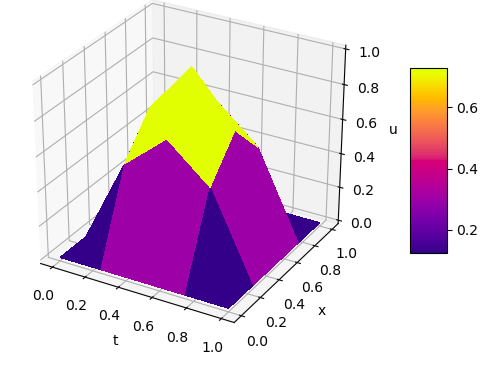
\includegraphics[width=1\linewidth]{img/u_real4.png} \\ а)}
	\end{minipage}
	\hfill
	\begin{minipage}[h]{0.49\linewidth}
		\center{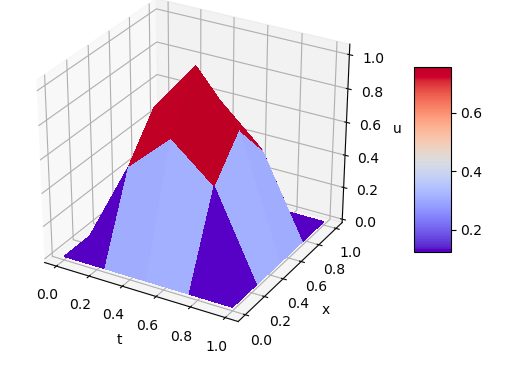
\includegraphics[width=1\linewidth]{img/u4.png} \\ б)}
	\end{minipage}
	\caption{a)решение системы, б)действительное значение при $n=4$}
	\label{ris:image1}
\end{figure}
\\
Значения минимального и максимального собственных чисел: 
\[
	Eigs:  27.38807021966818 \;\;100.61192978033175
\]
Ошибка выглядит следующим образом:
\\
\begin{figure}[h]
	\center{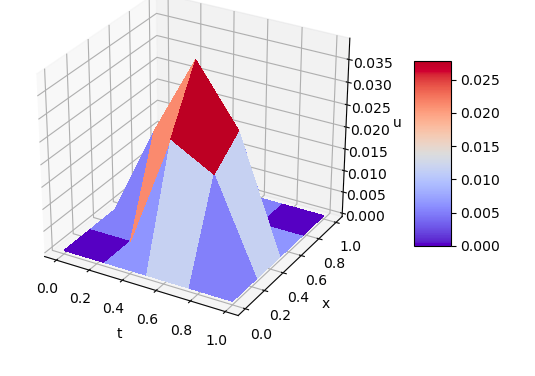
\includegraphics[width=0.5\linewidth]{img/error4.png}}
	\caption{ошибка при $n=4$}
	\label{ris:image}
\end{figure}
\newpage
При $h = 0.625$:
\\
Функция решения и действительная функция:
\\
\begin{figure}[h]
	\begin{minipage}[h]{0.49\linewidth}
		\center{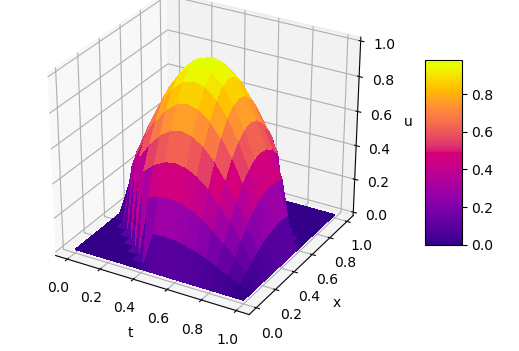
\includegraphics[width=1\linewidth]{img/u_real16.png} \\ а)}
	\end{minipage}
	\hfill
	\begin{minipage}[h]{0.49\linewidth}
		\center{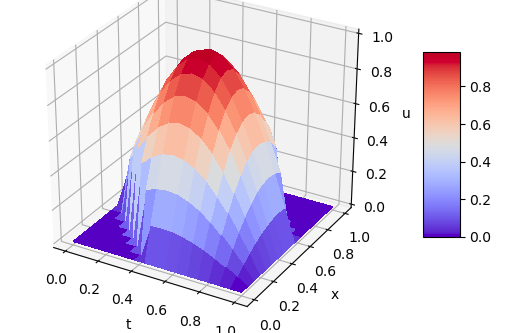
\includegraphics[width=1\linewidth]{img/u16.png} \\ б)}
	\end{minipage}
	\caption{a)решение системы, б)действительное значение при $n=16$}
	\label{ris:image1}
\end{figure}
\\
Значения минимального и максимального собственных чисел: 
\[
	Eigs:  31.841084906917786\;\;2016.1589150930836
\]
Ошибка выглядит следующим образом:
\\
\begin{figure}[h]
	\center{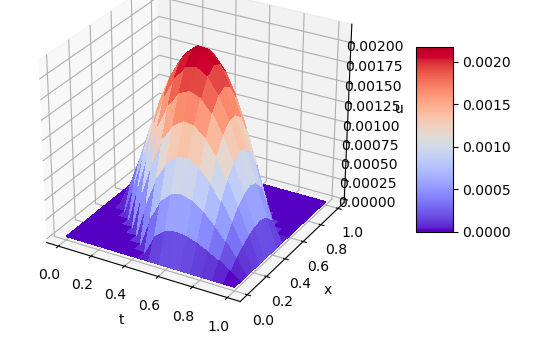
\includegraphics[width=0.5\linewidth]{img/error16.png}}
	\caption{ошибка при $n=16$}
	\label{ris:image}
\end{figure}
\\
Заметим, что во втором тесте мы увеличили $h$ в 4 раза и наша ошибка уменьшилась в 17,5 раз, даже лучше чем должна была (теоретически должна была уменьшиться в 16 раз).

\newpage
\section{Выводы.}

Таким образом мы исследовали задачу Дирихле в ограниченной области и изучили ход ее решения. Убедились в том, что при увеличении шага $h$, погрешность решения уменьшается примерно в $h^2$ раз.

Этот метод не очень прост в реализации: в нем участвуют сразу несколько дополнительных методов для поиска собственных чисел и решения системы линейных уравнений. Мы научились работать с упаковочными массивами, графически изображать решение и итерационно решать дифференциальные уравнения.

Таким образом,данный метод можно разными способами модифицировать, что также является плюсом метода.

\end{document}
